% Copyright (C) 2022
% School of Artificial Intelligence, Southeast University.
% --------------------------------------------------------------------------
%
% This work may be distributed and/or modified under the
% conditions of the LaTeX Project Public License, either
% version 1.3c of this license or (at your option) any later
% version. This version of this license is in
%    http://www.latex-project.org/lppl/lppl-1-3c.txt
% and the latest version of this license is in
%    http://www.latex-project.org/lppl.txt
% and version 1.3 or later is part of all distributions of
% LaTeX version 2005/12/01 or later.
%
% This work has the LPPL maintenance status `maintained'.
% The Current Maintainer of this work is xiangmin zhu.

\documentclass{seuthesis-2022}
\usepackage{amsmath}
\usepackage{gensymb}
\usepackage{listings}
\usepackage{float}
\numberwithin{equation}{section}

\title{基于六维力传感器的集装箱扭锁的}{机器人智能开合操作}

\studentnum{08119122}
\author{朱湘民}
\department{自动化学院}
\major{机器人工程}
\supervisor{李俊、陆坤}
\period{2022.12.15-2023.6.5}


\begin{document}

\maketitle
\makedeclaration

\frontmatter
\begin{abstract}[zh]
  摘要内容独立于正文而存在,是论文内容高度概括的简要陈述,应准确、具体、完整地概括论文的主要信息,内容包括研究目的、方法、过程、成果、结论及主要创新之处等,不含图表,不加注释,具有独立性和完整性,一般为400字左右。

  \keywords{关键词1,关键词2,关键词3,关键词4}
\end{abstract}

\begin{abstract}[en]
  英文摘要应与中文摘相对应,250个实词左右。采用第三人称介绍该学位论文内容,叙述的基本时态为一般现在时,确实需要强调过去的事情或者已经完成的行为才使用过去时、完成时等其他时态。

  \keywords{Keywords1,Keywords2,Keywords3,Keywords4}
\end{abstract}

\tableofcontents

\mainmatter
\chapter{绪论}
\section{课题背景和意义}
集装箱运输自20世纪50年代\cite{levinson2016box}开始出现,不断的发展至今,已经成为一种不可缺少的重要海上运输方式。
它具有多式联运、高效性、安全性、成本低和易管理等多方面的优点,使得其在全世界范围内成为国际贸易的主要运输方式。
2021年,欧美等疫情较为严重地区对电子产品、医疗物资、居家用品的进口需求持续增长,尤其在宽松货币政策与财税刺激政策助力下,国际商品贸易大幅反弹,使港口集装箱货运需求激增。
根据上海国际航运研究中心统计\cite{shanghai2022report},世界前100港口,我国占据28位,在2021全年,上海以4703万TEU的吞吐量位列世界第一。
随着集装箱行业的不断发展,装载率不断的提升,我们对集装箱自动化装卸技术的需求也在日益增加。

甲板上装载集装箱在海上运输往往会受到恶劣的天气影响,船舶的剧烈运动对作用在集装箱上的载荷影响更是巨大。
如果没有固定牢固,集装箱发生倾倒,将会产生巨大的损失。
因此对集装箱进行系固,限制其在船上的运动,对集装箱运输有重要意义。
在集装箱的四个角都安装有角件,正是通过角件与扭锁的连接,使得众多集装箱可以成为一个整体,更加稳固\cite{谢琛2015集装箱扭锁技术的现状及发展趋势}。

目前,扭锁安装在集装箱装卸过程中仍然主要依赖人工操作。尽管已经有一些自动化技术的应用,但在全球范围内,自动化扭锁安装,拆锁的普及程度相对较低。
扭锁对准安装,开锁以及解锁,是一系列重复性很强的简单操作,并且在码头生产岸线存在大量的安全隐患,船舶的废弃烟尘、流动的机械车辆以及高空坠物,严重影响了工人的身体健康。
国内外都曾经出现过多起扭锁安装过程中因存在安全隐患而造成的伤亡事故,造成了多方面的人身损失和财产损失\cite{平原2018机器人扭锁自动化装卸抓取规划研究}。
我们需要投入更多的研究和创新,以推动自动化扭锁一系列操作技术的发展和应用。

机器人技术在工业上的应用已经非常广泛,涵盖了生产、搬运、包装、协作以及数据分析等多个方面。
它们在提高效率、减少人工劳动、保障安全和提升生产质量方面发挥着重要的作用。
而在机器人领域中,感知方面一直是研究重点,要实现对机器人的控制,它首先要具备对环境的交互以及感知能力。
由于六维力传感器能够在三维空间中测量在三个坐标轴上的力,即X轴、Y轴和Z轴的力与力矩的大小,所以在机器人中成为了最常用的传感器之一。
例如:通过实时测量机器人与周围环境之间的力,机器人可以调整自身力的施加,实现精确的力控制和力反馈

在机器人与集装箱扭锁接触的过程中,对于集装箱的扭锁进行柔顺、平稳的操作。
如果仅采用简单的位置控制,可能会造成很大的误差,对于机器人这种刚度很高的结构,微小的位置误差都可能会造成很大的作用力,最终导致严重的后果,所以为了实现机器人扭锁开合操作,机器人需要表现出柔顺性。
柔顺控制是指机器人以柔软和灵活的方式与周围环境进行交互和操作的控制策略,使其具备人的智能,从而可以在严苛的环境中进行工作。

基于六维力传感器的柔顺控制主要从力传感器获得力和力矩的信息,再将其转换为机器人的控制信号,使得机器人做出对应的动作。柔顺控制主要分为主动柔顺控制和被动柔顺控制。
被动柔顺控制就是在机械臂末端再安装一个机械弹性结构,通过机械臂的弹性来实现力控功能。主动柔顺则是依靠控制策略在机器人末端产生需要的刚度、阻尼或力以达到柔顺控制的作用。
在实际生产需求当中,被动柔顺控制方法简单,成本低廉,对机械臂无特殊要求,但是由于力控精度无法保证,无法确保不会出现很大的接触力导致机械臂损坏。
所以采用基于六维力传感器的主动柔顺控制具有重要的意义。

采用主动柔顺控制对扭锁进行开合操作有很多优点,过度使用力量和速度开锁和锁紧集装箱可能导致扭锁、和其他机械部件的损坏,增加设备维修和更换的频率。
通过实施柔顺控制,可以减少扭锁的损耗,延长扭锁的使用寿命,降低维护成本,这对于现代物流运输行业的发展和提升整体运输效能具有重要意义。

我们团队分为四个课题针对集装箱扭锁进行自动化处理,其中三个课题对视觉部分进行处理,检测锁孔的位置并对准,检测扭锁以及锁杆的位姿。
本课题主要负责力控部分,使用机器人对确定好位姿的扭锁连杆进行柔顺控制开合操作。
通过扭锁操作自动化提高生产效率、降低成本、提升产品质量和减少人力劳动的需求。它是现代制造业中追求高效、精确和可持续发展的重要手段之一。

\section{国内外研究现状}



\section{本文研究内容}

\chapter{控制器系统整体研究方案}

\section{控制系统总体方案}

\section{系统硬件选型}

\section{控制系统软件架构}

\section{六维力传感器数据补偿}




\chapter{机器人运动学研究}
为实现机器人的柔顺控制,运动控制\cite{niku2020introduction}是最基础的部分。
运动控制主要的研究问题在于机器人各个关节所处的空间位置,即机器人末端执行器与各个关节变量之间的关系。
其中,正运动学在于已知机器人的构型,根据给定的连杆长度与关节角度去计算机器人末端执行器的位姿;
逆运动学则是根据给定的机器人末端执行器的位姿来确定每个关节的角度。

本章将对UR5机器人进行运动学分析,介绍机器人的坐标变换;建立机器人连杆坐标系;求解机器人正逆运动学问题;仿真验证机器人运动学正逆解的正确性。

\section{空间变换与描述}
在机器人控制过程中,我们首先要对机器人的运动学进行分析和求解。
整个机器人的运动学研究都基于其所处的坐标系和坐标系变换。
\setcounter{equation}{0}

\subsection{位置描述}
我们在坐标系\{$A$\}中对矢量$^{A}P$进行表示
\begin{equation}
^{A}P = 
\begin{bmatrix}
  P_{x}\\P_{y}\\P_{z}
\end{bmatrix}
\end{equation}
用上述的有序三元组对我们在的空间质点进行表示,这三个点是独立的,因此具有3个自由度。

\subsection{姿态描述}
在位置描述中,我们关心的对象是一个质点,它本身不具有姿态的信息,所以没有引入旋转,但是当我们研究的对象是机器人这样的刚体时,我们需要在刚体上固定一个坐标系,用来表示刚体的旋转。
如图所示,我们对机器人末端手爪中心的位姿进行表示,在坐标系\{$A$\}中,以该点为原点选择三个正交向量作为轴,建立坐标系\{$B$\}。
此时我们就可以分别用$X_{A}$、$Y_{A}$、$Z_{A}$和$X_{B}$、$Y_{B}$、$Z_{B}$来表示坐标系\{$A$\}和坐标系\{$B$\}的主轴基矢量,
并定义旋转矩阵$^{A}_{B}R$表示\{$B$\}相对于\{$A$\}的旋转矩阵
\begin{equation}
^{A}_{B}R = 
\begin{bmatrix}
  ^{A}\hat{X}_{B} & ^{A}\hat{Y}_{B} & ^{A}\hat{Z}_{B}
\end{bmatrix}
=
\begin{bmatrix}
  \hat{X}_{B} \cdot \hat{X}_{A} & \hat{Y}_{B} \cdot \hat{X}_{A} & \hat{Z}_{B} \cdot \hat{X}_{A}\\
  \hat{X}_{B} \cdot \hat{Y}_{A} & \hat{Y}_{B} \cdot \hat{Y}_{A} & \hat{Z}_{B} \cdot \hat{Y}_{A}\\
  \hat{X}_{B} \cdot \hat{Z}_{A} & \hat{Y}_{B} \cdot \hat{Z}_{A} & \hat{Z}_{B} \cdot \hat{Z}_{A}\\
\end{bmatrix}
\end{equation}

另一方面$^{B}_{A}R$表示\{$A$\}相对于\{$B$\}的旋转矩阵
\begin{equation}
^{A}_{B}R = 
\begin{bmatrix}
  ^{B}\hat{X}_{A} & ^{B}\hat{Y}_{A} & ^{B}\hat{Z}_{A}
\end{bmatrix}
=
\begin{bmatrix}
  ^{A}\hat{X}^{T}_{B}\\
  ^{A}\hat{Y}^{T}_{B}\\
  ^{A}\hat{Z}^{T}_{B}\\
\end{bmatrix}
\end{equation}

旋转矩阵的性质如下:
\begin{equation}
\begin{cases}
  ^{A}_{B}R = ^{B}_{A}R^{T}\\
  ^{A}_{B}R \cdot ^{B}_{A}R = I\\
  ^{A}_{B}R = ^{B}_{A}R^{-1}\\
\end{cases}
\end{equation}

在机器人学中,位置与姿态通常成对出现,将其组合起来称之为坐标系,例如坐标系\{$B$\}在坐标系\{$A$\}中表示如下:
\begin{equation}
\{B\}=\{^{A}_{B}R,^{A}P_{BORG}\}
\end{equation}

\subsection{坐标系的映射}
主要分为平移坐标系的映射,旋转坐标系的映射和一般坐标系的映射。

\begin{itemize}
  \item [(1)]
  平移坐标系的映射

  当\{$B$\}与\{$A$\}以相同的姿态出现,但是原点不同时,则$B$相对于$A$的位置可以表示为:
  \begin{equation}
  ^{A}P=^{B}P+^{A}P_{BORG}
  \end{equation}
  
  \item [(2)]旋转坐标系的映射
  
  当\{$A$\}与\{$B$\}的原点重合,\{$A$\}相对于\{$A$\}的$z$轴旋转$\theta$得到的,我们假设存在$^{B}P$点位于\{$B$\}中,我们通过计算推出$^{B}P$点在\{$A$\}中的投影分别为:
  \begin{equation}
    ^{A}P_x = {^{B}\hat{X}^{T}_{A}} \cdot {^{B}P}
  \end{equation}
  \begin{equation}
    ^{A}P_y = {^{B}\hat{Y}^{T}_{A}} \cdot {^{B}P}
  \end{equation}
  \begin{equation}
    ^{A}P_z = {^{B}\hat{Z}^{T}_{A}} \cdot {^{B}P}
  \end{equation}

  简化后得到:
  \begin{equation}
  ^{A}P = {^{B}_{A}R} {^{B}P}
  \end{equation}
  此时我们可以推出基本旋转矩阵(绕$z$轴旋转)记为$R(z,0)$。
  \begin{equation}
  R(z,0) = ^{B}_{A}R =
  \begin{bmatrix}
    cos\theta & -sin\theta & 0\\
    sin\theta & cos\theta & 0\\
    0 & 0 & 1\\
  \end{bmatrix}
\end{equation}
  同理,我们推出绕$x$、$y$轴旋转的基本旋转矩阵
  \begin{equation}
  R(x,0) =
  \begin{bmatrix}
    1 & 0 & 0\\
    0 & cos\theta & -sin\theta\\
    0 & sin\theta & cos\theta\\
  \end{bmatrix}
  \end{equation}
  \begin{equation}
  R(y,0) =
  \begin{bmatrix}
    cos\theta & 0 & sin\theta\\
    0 & 1 & 0\\
    -sin\theta & 0 & cos\theta\\
  \end{bmatrix}
  \end{equation}
  \item [(3)]
  考虑一般情况,\{$B$\}与\{$A$\}原点不同且姿态有偏差,
  此时按照平移映射中的结论,如果应用向量加法求得点$^{B}P$在\{$A$\}中表示 ,前提是\{$B$\}相对于\{$A$\}没有旋转
  所以我们需要先绕\{$B$\}的原点旋转,使其与\{$A$\}的姿态一致,记为坐标系\{$C$\}。此时$P$在\{$C$\}中表示为${^{C}_{B}R} \cdot {^{B}P}$
  而\{$C$\}与\{$A$\}的姿态一致,${^{A}_{B}R} \cdot {^{B}P} = {^{C}_{B}R} \cdot {^{B}P}$
  我们得到了如下的等式:
  \begin{equation}
  \begin{aligned}
    ^{A}P &= {^{A}_{C}R} \cdot {^{C}P} + {^{A}P_{CORG}}\\
          &= {^{A}_{C}R} \cdot ({^{C}_{B}R} \cdot {^{B}P} + {^{C}P_{BORG}}) + {^{A}P_{BORG}}\\
          &= I \cdot ({^{C}_{B}R} \cdot {^{B}P} + 0) + {^{A}P_{BORG}}\\
          &= {^{A}_{B}R} \cdot {^{B}P} + {^{A}P_{BORG}}\\
  \end{aligned}
  \end{equation}
  为更加简洁的表示该公式,我们将其表示为$4 \times 4$的矩阵:
  \begin{equation}
  \begin{bmatrix}
    ^{A}P\\
    1\\
  \end{bmatrix}
  =
  \begin{bmatrix}
    ^{A}_{B}R & ^{A}P_{BORG}\\
    \vec{0} & 1\\
  \end{bmatrix}
  \begin{bmatrix}
    ^{B}P\\
    1\\
  \end{bmatrix}
  \end{equation}
  定义齐次变换矩阵为:
  \begin{equation}\label{eq:1}
  ^{A}_{B}T =
  \begin{bmatrix}
    ^{A}_{B}R & ^{A}P_{BORG}\\
    \vec{0} & 1\\
  \end{bmatrix}
  \end{equation}
\end{itemize}


\section{连杆参数与连杆坐标系}
机器人一般由多个关节和连杆构成,从机械臂的$Base\_link$开始,依次对连杆进行编号。
本文研究的对象为Universal Robots公司生产的UR5工业机器人,它共有六个自由度,具有6个独立的关节,且全部为转动关节,可以看作由转动关节串联的连杆组成的
为了便于处理,我们在机器人每个关节上建立连杆坐标系

\subsection{连杆坐标系的建立}
本文选择Denavit和Hartenberg于1955年提出一种针对串联机械臂连杆和关节的数学建模方法\cite{1955A}。
以机器人的基座为连杆0开始对连杆编号,第一个可动连杆为连杆1,依次排序,根据D-H建模方法建立坐标系需要保证以下原则:
\begin{itemize}
  \item[(1)]
  $Z_i$轴沿着第$i+1$个关节的转轴方向,其中方向的不同会影响连杆的转动方向,由右手定则判定。
  \item[(2)]
  坐标系$i$原点$O_i$在连杆$i$的末端位置,$Z_i$和$Z_{i+1}$的公共法线与$Z_{i+1}$的交点处;
  如果$Z_i$和$Z_{i+1}$相交,则原点$O_i$定在交点处,即关节的中心处。
  \item[(3)]
  $X_i$轴同时垂直于$Z_i$和$Z_{i-1}$,即公共法线;如果$Z_i$和$Z_{i+1}$相交,则垂直与两者确定的平面,方向有两种选择。
  \item[(4)]  
  $Y_i$轴的方向根据右手定则确定。
\end{itemize}

对各个连杆建立坐标系之后,通过平移和旋转来进行坐标系$\{i-1\}$到坐标系$\{i\}$的转换,步骤如下:

\begin{itemize}
  \item [(1)]
  将坐标系$\{i-1\}$绕$z_{i}$轴旋转$\theta$角,使得$x_{i-1}$与$x_{i}$互相平行
  \item [(2)]
  沿$z_{i}$平移$d_{i}$的距离,使得使得$x_{i-1}$与$x_{i}$轴重合
  \item [(3)]
  沿$x_{i-1}$平移$a_{i}$的距离,使得坐标系$\{i-1\}$与坐标系$\{i\}$的原点重合
  \item [(4)]
  令$z_{i-1}$轴沿着$x_{i-1}$旋转$\alpha_i$,使得两坐标系重合;
\end{itemize}

上述每个步骤对应的齐次变换矩阵我们可以根据公式\eqref{eq:1}给出:
\begin{equation}
  Rot(z_{i},\theta_{i})=
  \begin{bmatrix}
    cos\theta_{i} & -sin\theta_{i}& 0 & 0\\
    sin\theta_{i} & cos\theta_{i} & 0 & 0\\
    0 & 0 & 1 & 0\\
    0 & 0 & 0 & 1\\
  \end{bmatrix}
\end{equation}

\begin{equation}
  Trans(z_{i},d_{i})=
  \begin{bmatrix}
    1 & 0 & 0 & 0\\
    0 & 1 & 0 & 0\\
    0 & 0 & 1 & d_i\\
    0 & 0 & 0 & 1\\
  \end{bmatrix}
\end{equation}

\begin{equation}
  Trans(x_{i},a_{i})=
  \begin{bmatrix}
    1 & 0 & 0 & a_{i}\\
    0 & 1 & 0 & 0\\
    0 & 0 & 1 & 0\\
    0 & 0 & 0 & 1\\
  \end{bmatrix}
\end{equation}

\begin{equation}
  Rot(x_{i},\alpha_{i})=
  \begin{bmatrix}
    1 & 0 & 0 & 0\\
    0 & cos\alpha_{i} & sin\alpha_{i} & 0\\
    0 & sin\alpha_{i} & cos\alpha_{i} & 0\\
    0 & 0 & 0 & 1\\
  \end{bmatrix}
\end{equation}

因此,坐标系$\{i-1\}$到坐标系$\{i\}$的的齐次坐标变换矩阵为:
\begin{equation}\label{eq:坐标系间变换}
\begin{aligned}
  ^{i-1}_{i}T &=Rot(z_{i},\theta_{i})Trans(z_{i},d_{i})Trans(x_{i-1},a_{i-1})Rot(x_{i},\alpha_{i})\\
              &=\begin{bmatrix}
                  cos\theta_{i} & -sin\theta_{i}cos\alpha_{i} & sin\theta_{i}sin\alpha_{i} & a_{i}cos\theta_{i}\\
                  sin\theta_{i} & cos\theta_{i}cos\alpha_{i} & -cos\theta_{i}sin\alpha_{i} & a_{i}sin\theta_{i}\\
                  0 & sin\alpha_{i} & cos\alpha_{i} & d_{i}\\
                  0 & 0 & 0 & 1\\
                \end{bmatrix}
\end{aligned}
\end{equation}



\subsection{UR5机器人运动学模型}
通过官方文档下载UR5SolidWorks模型文件并导入,获得UR5机器人模型及参数如图\ref{fig:UR5型机器人结构}所示:
\begin{figure}[H]
  \centering
  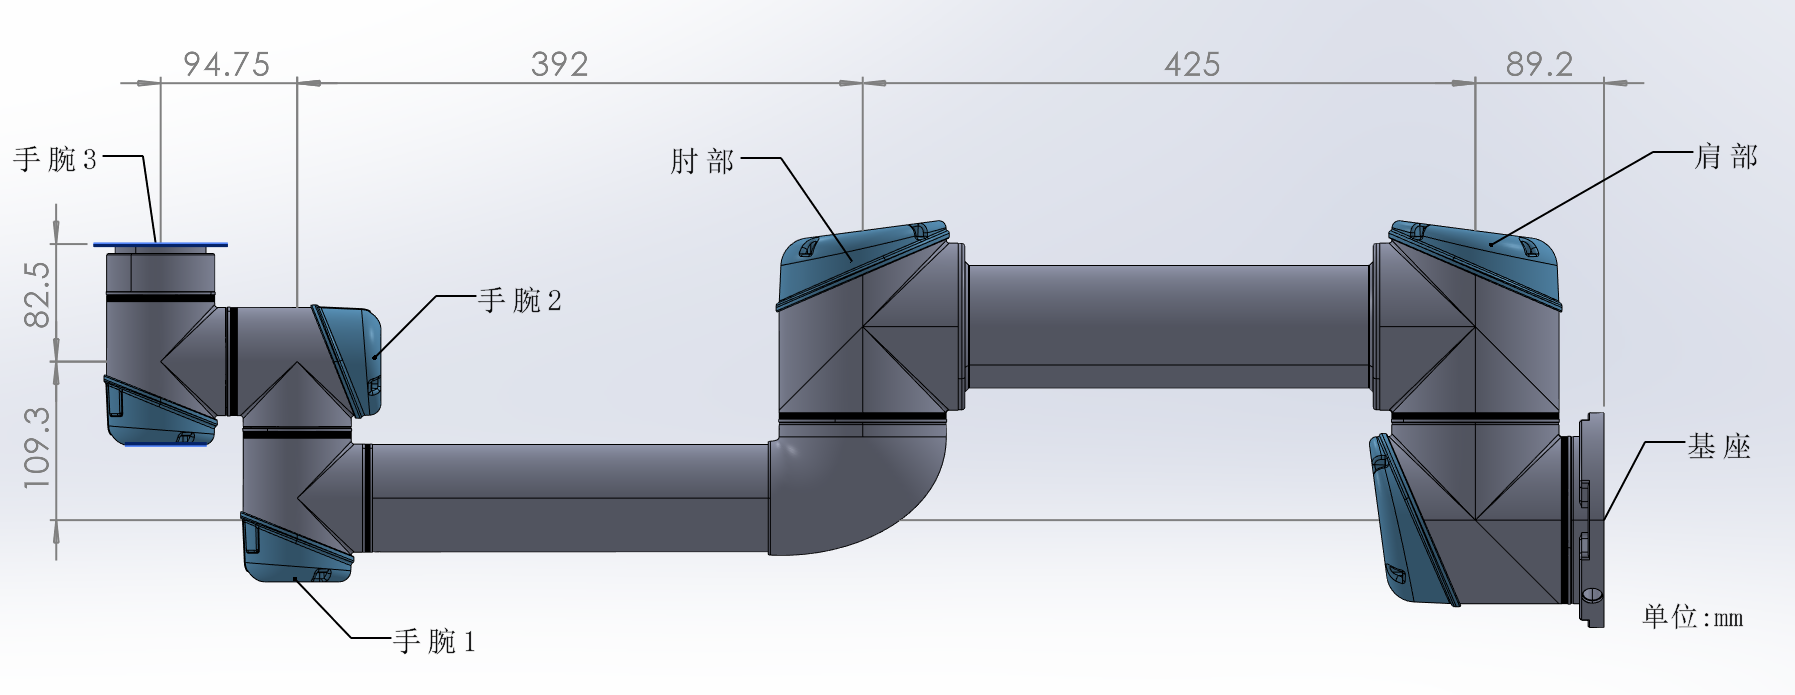
\includegraphics[width=1.0\linewidth]{fig/UR5型机器人结构.png}
  \caption{UR5型机器人结构}
  \label{fig:UR5型机器人结构}
\end{figure}
按照D-H建模原则,建立UR5坐标系如图\ref{fig:UR5_DH参数}
\begin{figure}[H]
  \centering
  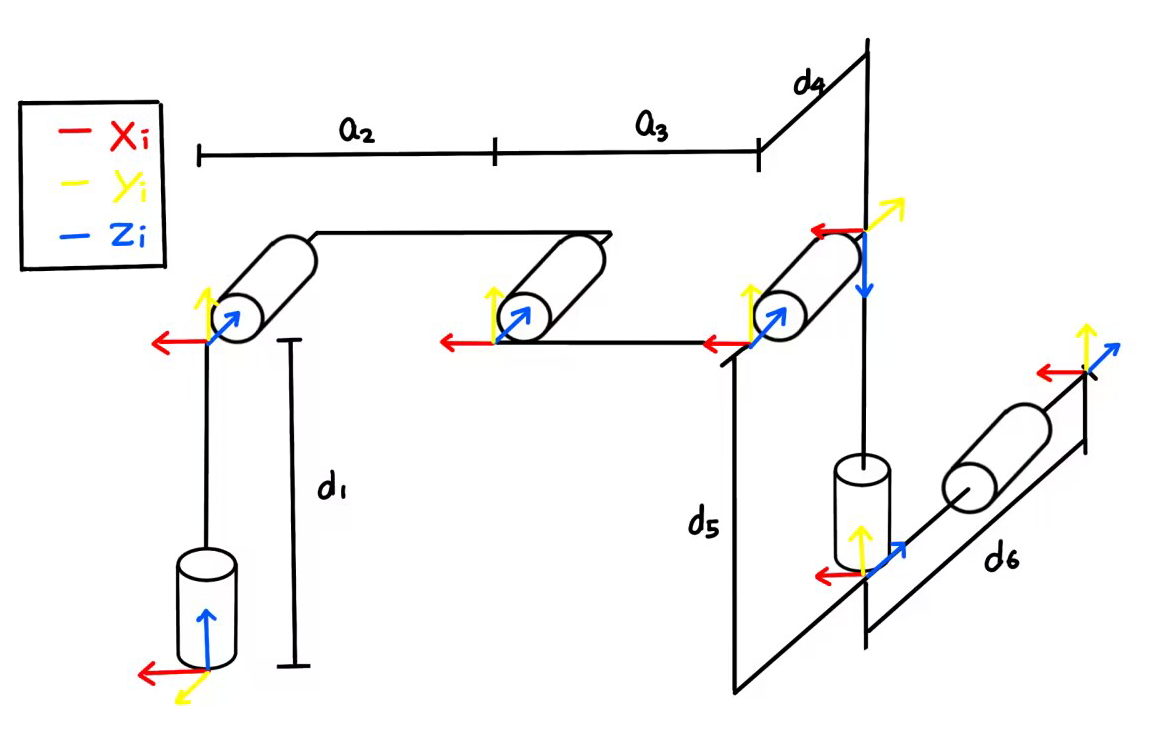
\includegraphics[width=1.0\linewidth]{fig/UR5_DH参数.png}
  \caption{UR5机器人坐标系示意图}
  \label{fig:UR5_DH参数}
\end{figure}
UR5机器人DH参数表如下
\begin{table}[H]
  \centering
  \caption{UR5机器人D-H参数表}
  \label{tab:UR5机器人D-H参数表}
  \small
  \begin{tabular}{ccccc}
    \toprule
    连杆 & 连杆距离$d_{i}$/$mm$ & 连杆长度$a_{i}$/$mm$& 连杆扭角$\alpha$/(\degree) & 连杆转角$\theta_{i}$/(\degree)\\
    \midrule
    1 & $d_{1}=89.2$ & $0$ & $\pi/2$ & $\theta_{1}$\\
    2 & $0$ & $a_{2}=-425$ & $0$ & $\theta_{2}$\\
    3 & $0$ & $a_{3}=-392$ & $0$ & $\theta_{3}$\\
    4 & $d_{4}=109.3$ & $0$ & $\pi/2$ & $\theta_{4}$\\
    5 & $d_{5}=94.75$ & $0$ & $-\pi/2$ & $\theta_{5}$\\
    6 & $d_{6}=82.5$ & $0$ & $0$ & $\theta_{6}$\\
    \bottomrule
  \end{tabular}
\end{table}

\section{正运动学求解}\label{正运动学}
为得到UR5机械臂的末端关节位姿,我们需要从前一关节转换到下一关节,设已知坐标系为$\{i-1\}$,通过平移和旋转将$\{i-1\}$转换到$\{i\}$。
结合表\ref{tab:UR5机器人D-H参数表}和公式\eqref{eq:坐标系间变换},在UR5机器人的D-H参数变换中,只有$\theta$一个参数,我们做如下简化,定义$s_i=sin\theta_i$,$c_i=cos\theta_i$,$\theta_{ij} = \theta_i + \theta_j$,
$s_{ij} = sin(\theta_i+\theta_j)$,$c_{ij} = cos(\theta_i+\theta_j)$,以此类推。

相邻连杆之间的变换矩阵为:
\begin{equation}
  ^0_1T(\theta_1)=
  \begin{bmatrix}
    c_1 & 0 & s_1 & 0\\
    s_1 & 0 & -c_1 & 0\\
    0 & -1 & 0 & d_1\\
    0 & 0 & 0 & 1\\
  \end{bmatrix}
  \label{eq:^0_1T}
\end{equation}

\begin{equation}
  ^1_2T(\theta_2)=
  \begin{bmatrix}
    c_2 & -s_2 & 0 & a_2c_2\\
    s_2 & c_2 & 0 & -a_2s_2\\
    0 & 0 & 1 & 0\\
    0 & 0 & 0 & 1\\
  \end{bmatrix}
  \label{eq:^1_2T}
\end{equation}

\begin{equation}
  ^2_3T(\theta_3)=
  \begin{bmatrix}
    c_3 & -s_3 & 0 & a_3c_3\\
    s_3 & c_3 & 0 & a_3s_3\\
    0 & -1 & 0 & 0\\
    0 & 0 & 0 & 1\\
  \end{bmatrix}
  \label{eq:^2_3T}
\end{equation}

\begin{equation}
  ^3_4T(\theta_4)=
  \begin{bmatrix}
    c_4 & 0 & s_4 & 0\\
    s_4 & 0 & -c_4 & 0\\
    0 & 1 & 0 & d_4\\
    0 & 0 & 0 & 1\\
  \end{bmatrix}
  \label{eq:^3_4T}
\end{equation}

\begin{equation}
  ^4_5T(\theta_5)=
  \begin{bmatrix}
    c_5 & 0 & -s_5 & 0\\
    s_5 & 0 & c_5 & 0\\
    0 & -1 & 0 & d_5\\
    0 & 0 & 0 & 1\\
  \end{bmatrix}
  \label{eq:^4_5T}
\end{equation}

\begin{equation}
  ^5_6T(\theta_6)=
  \begin{bmatrix}
    c_6 & -s_6 & 0 & 0\\
    s_6 & c_6 & 0 & 0\\
    0 & 0 & 1 & d_6\\
    0 & 0 & 0 & 1\\
  \end{bmatrix}
  \label{eq:^5_6T}
\end{equation}

针对UR5机器人,求其末端执行器所在的坐标系,我们可以利用相邻的连杆坐标系间的齐次变换矩阵相乘,最终得到末端执行器的变换矩阵为:
\begin{equation}
  ^0_6T={^0_1T}{^1_2T}{^2_3T}{^3_4T}{^4_5T}{^5_6T}=
  \begin{bmatrix}
    n_x & o_x & a_x & p_x\\
    n_y & o_y & a_y & p_y\\
    n_z & o_z & a_z & p_z\\
    0 & 0 & 0 & 1\\
  \end{bmatrix}
  \label{eq:^0_6T}
\end{equation}

其中具体公式如下:($s_{ij}=sin(a_i+a_j)$,$c_{ij}=cos(a_i+a_j)$)
\begin{equation}
  \begin{aligned}
    &n_x = c_6(c_1c_{23}s_5+c_5s_1s_4+c_1c_2c_4c_5s_3+c_1c_3c_4c_5s_2) - s_6(c_1c_2s_3s_4-c_4s_1+c_1c_3s_2s_4)\\
    &o_x = -c_6(c_1c_2s_3s_4-c_4s_1+c_1c_3s_2s_4) - s_6(c_1c_{23}s_5+c_5s_1s_4+c_1c_2c_4c_5s_3+c_1c_3c_4c_5s_2)\\
    &a_x = c_1c_5c_{23} - s_5(s_1s_4+c_1c_2c_4s_3+c_1c_3c_4s_2)\\
    &\begin{split}
      p_x = &c_1a_1+c_1s_2a_2+c_1c_2c_3d_4+c_1c_2s_3a_3+c_1c_3s_2a_3-c_1s_2s_3d_4-s_1s_4s_5d_6\\
            &+c_1c_2c_3c_5d_6-c_1c_5s_2s_3d_6-c_1c_2c_4s_3s_5d_6-c_1c_3c_4s_2s_5d_6\\
     \end{split}\\
    &n_y = c_6(c_{23}s_1s_5-c_1c_5s_4+c_2c_4c_5s_1s_3+c_3c_4c_5s_1s_2) - s_6(c_1c_4+c_2c_1s_3s_4+c_3s_1s_2s_4)\\
    &o_y = -c_6(c_1c_4+c_2s_1s_3s_4+c_3s_1s_2s_4) - s_6(c_{23}s_1s_5-c_1c_5s_4+c_2c_4c_5s_1s_3+c_3c_4c_5s_1s_2)\\
    &a_y = c_5c_{23}s_1 - s_5(c_2c_4s_1s_3-c_1s_4+c_3c_4s_1s_2)\\
    &\begin{split}
      p_y = &s_1a_1 + s_1s_2a_2 + c_2c_3s_1d_4 + c_2s_1s_3a_3 + c_3s_1s_2a_3 + c_1s_4s_5d_6 - s_1s_2s_3d_4\\
            &+c_2c_3c_5s_1d_6 - c_5s_1s_2s_3d_6 - c_2c_4s_1s_3s_5d_6 - c_3c_4s_1s_2s_5d_6\\
     \end{split}\\ 
    &n_z = -c_6(s_5s_{23}-c_4c_5c_{23}) - c_{23}s_4s_6\\
    &o_z = s_6(s-5s_{23}-c_4c_5c_{23}) - c_6c_{23}s_4\\ 
    &a_z = -c_5c_{23} - c_4c_{23}s_5\\
    &\begin{split}
      p_z = &d_1 + c_2a_2 + c_2c_3a_3 - c_2s_3d_4 + c_3s_2d_4 + s_2s_3a_3 - c_2c_5s_3d_6 - c_3c_5s_2d_6\\
            &- c_2c_3c_4s_5d_6 + c_4s_2s_3s_5d_6\\
     \end{split}
  \end{aligned} 
\end{equation}


\section{逆运动学求解}\label{逆运动学}
UR5逆运动学方程是指根据机器人末端执行器相对于基座的位姿,运用反变换的方法,对正运动学进行逆向求解的过程,通过此方法可以求出机器人各个关节变量$\theta_i$。

假定末端位姿已知,且为$^0_6T$,由公式\eqref{eq:^0_6T}给出。

\subsection{对关节1、5、6进行求解:}
由公式\eqref{eq:^0_1T}和公式\eqref{eq:^5_6T}可知
\begin{equation}
  ^0_1T^{-1}=
  \begin{bmatrix}
    c_1 & s_1 & 0 & 0\\
    0 & 0 & 1 & -d_1\\
    s_1 & -c_1 & 0 & 0\\
    0 & 0 & 0 & 1\\
  \end{bmatrix}
  \label{eq:^0_1T^{-1}}
\end{equation}

\begin{equation}
  ^5_6T^{-1}=
  \begin{bmatrix}
    c_6 & s_6 & 0 & 0\\
    -s_6 & c_6 & 0 & 0\\
    0 & 0 & 1 & -d_6\\
    0 & 0 & 0 & 1\\
  \end{bmatrix}
  \label{eq:^5_6T^{-1}}
\end{equation}

对$^0_6T$依次左乘$^0_1T^{-1}$,右乘$^5_6T^{-1}$,得到:
\begin{equation}
  {^0_1T^{-1}} {^0_6T} {^5_6T^{-1}} =
  \begin{bmatrix}
    A_{11} & A_{12} & A_{13} & A_{14}\\
    A_{21} & A_{22} & A_{23} & A_{24}\\
    A_{31} & A_{32} & A_{33} & A_{34}\\
    0 & 0 & 0 & 1\\
  \end{bmatrix}
  \label{eq:^1_5T逆}
\end{equation}

其中:

$A_{11} = c_6(n_xc_1+n_ys_1)-s_6(o_xc_1+o_ys_1)$

$A_{12} = s_6(n_xc_1+n_ys_1)+c_6(o_xc_1+o_ys_1)$

$A_{13} = a_xc_1+a_ys_1$

$A_{14} = p_xc_1-d_6(a_xc_1+a_ys_1)+p_ys_1$

$A_{21} = n_xc_6-o_zs_6$

$A_{22} = o_zc_6+n_zs_6$

$A_{23} = a_z$

$A_{24} = p_z-d_1-a_zd_6$

$A_{31} = s_6(o_yc_1-o_xs_1)-c_6(n_yc_1-n_xs_1)$

$A_{32} = -s_6(n_yc_1-n_xs_1)-c_6(o_yc_1-o_xs_1)$

$A_{33} = a_xs_1-a_yc_1$

$A_{34} = -p_yc_1+d_6(a_yc_1-a_xs_1)+p_xs_1$

将公式\eqref{eq:^0_6T}和代入公式\eqref{eq:^1_5T逆}通过计算可得:
\begin{equation}
  {^0_1T^{-1}} {^0_6T} {^5_6T^{-1}} = {^0_1T^{-1}} {^0_1T} {^1_2T} {^2_3T} {^3_4T} {^4_5T} {^5_6T}{^5_6T^{-1}} = ^1_5T
  \label{eq:^1_5T=^1_5T}
\end{equation}

又因为:
\begin{equation}
  ^1_5T = {^1_2T} {^2_3T} {^3_4T} {^4_5T} =
  \begin{bmatrix}
    c_{234}c_5 & -s_{234} & -c_{234}s_5 & a_3c_{23}+a_2c_2+d_5s_{234}\\
    s_{234}c_5 & c_{234} & -s_{234}s_5 & a_3s_{23}+a_2s_2-d_5c_{234}\\
    s_5 & 0 & c_5 & d_4\\
    0 & 0 & 0 & 1\\
  \end{bmatrix}
  \label{eq:^1_5T}
\end{equation}

由公式\eqref{eq:^1_5T=^1_5T}可知,等式两边矩阵相等,对应矩阵各个元素相等,故我们可以利用该等式求解关节角度。
\begin{itemize}
  \item [(1)]
  求解关节角$\theta_1$

  利用矩阵元素$A_{34}$结合公式\eqref{eq:^1_5T}
  \begin{equation}
    -p_yc_1+d_6(a_yc_1-a_xs_1)+p_xs_1 = d_4
  \end{equation}
  整理可得:
  \begin{equation}
    (d_6a_y-p_y)c_1 - (a_xd_6-p_x)s_1 = d_4
  \end{equation}
  解得:
  \begin{equation}
    \theta_1 = atan2(d_6a_y-p_y,a_xd_6-p_x)-atan2(d_4,\pm \sqrt[2]{(d_6a_y-p_y)^2+(a_xd_6-p_x)^2-{d_4}^2} )
  \end{equation}
  (其中$(d_6a_y-p_y)^2+(a_xd_6-p_x)^2-{d_4}^2 \geq 0$)
  \item [(2)]
  求解关节角$\theta_5$

  利用矩阵元素$A_{33}$结合公式\eqref{eq:^1_5T}
  \begin{equation}
    a_xs_1-a_yc_1 = c_5
  \end{equation}
  解得:
  \begin{equation}
    \theta_5 = \pm arccos(a_xs_1-a_yc_1)
  \end{equation}
  (其中$a_xs_1-a_yc_1 \leq 1$)
  \item [(3)]
  求解关节角$\theta_6$

  利用矩阵元素$A_{31}$结合公式\eqref{eq:^1_5T}
  \begin{equation}
    s_6(o_yc_1-o_xs_1)-c_6(n_yc_1-n_xs_1)=s_5
  \end{equation}
  整理得:
  \begin{equation}
    (n_xs_1-n_yc_1)c_6 - (o_xs_1-o_yc_1)s_6 = s_5
  \end{equation}
  解得:
  \begin{equation}
    \begin{aligned}
      \theta_6 = &atan2(n_xs_1-n_yc_1,o_xs_1-o_yc_1)\\
                  &-atan2(s_5,\pm \sqrt[2]{(n_xs_1-n_yc_1)^2+(o_xs_1-o_yc_1)^2-{s_5}^2})
    \end{aligned}
  \end{equation}
  通过化简我们可以求得:
  \begin{equation}
    (n_xs_1-n_yc_1)^2+(o_xs_1-o_yc_1)^2-{s_5}^2 = 0
  \end{equation}
  所以:
  \begin{equation}
    \theta_6 = atan2(n_xs_1-n_yc_1,o_xs_1-o_yc_1)-atan2(s_5,0) = atan2(\frac{n_xs_1-n_yc_1}{s_5},\frac{o_xs_1-o_yc_1}{s_5})
  \end{equation}
  (其中$s_5 \neq 0$)
\end{itemize}
  
  

\subsection{对关节2、3、4进行求解}
由公式\eqref{eq:^4_5T}可以求得:
\begin{equation}
  ^4_5T^{-1} =
  \begin{bmatrix}
    c_5 & s_5 & 0 & 0\\
    0 & 0 & -1 & d_5\\
    -s_5 & c_5 & 0 & 0\\
    0 & 0 & 0 & 1\\
  \end{bmatrix}
\end{equation}

对公式\eqref{eq:^1_5T逆}右乘$^4_5T^{-1}$得到:
\begin{equation}
  \begin{aligned}
    &{^0_1T^{-1}} {^0_6T} {^5_6T^{-1}} {^4_5T^{-1}} =
    &\begin{bmatrix}
      B^1_1 & B^1_2 & B^1_3 & B^1_4\\
      B^2_1 & B^2_2 & B^2_3 & B^2_4\\
      B^3_1 & B^3_2 & B^3_3 & B^3_4\\
      0 & 0 & 0 & 1\\
    \end{bmatrix}
  \end{aligned}
  \label{eq:^1_4T逆}
\end{equation}

其中:

$B_{11} = -c_5\left(s_6(o_xc_1+o_ys_1)-c_6(n_xc_1+n_ys_1)\right) - s_5(a_xc_1+a_ys_1)$

$B_{12} = c_5(a_xc_1+a_ys_1) - s_5\left(s_6(o_xc_1+o_ys_1)-c_6(n_xc_1+n_ys_1)\right)$

$B_{13} = -s_6(n_xc_1+n_ys_1)-c_6(o_xc_1+o_ys_1)$

$B_{14} = d_5\left(s_6(n_xc_1+n_ys_1)-c_6(o_xc_1+o_ys_1)\right) - d_5(a_xc_1+p_ys_1) + p_xc_1 + p_ys_1$

$B_{21} = c_5(n_xc_6-o_zs_6) - a_zs_5$

$B_{22} = s_5(n_zc_6-o_zs_6) + a_zs_5$

$B_{23} = -o_zc_6 - n_zs_6$

$B_{24} = p_z-d_1-a_zd_6 +d_5(o_zc_6+n_zs_6)$

$B_{31} = c_5\left(s_6(o_yc_1-o_xs_1)-c_6(n_yc_1-n_xs_1)\right) + s_5(a_yc_1-a_xs_1)$

$B_{32} = s_5\left(s_6(o_yc_1-o_xs_1)-c_6(n_yc_1-n_xs_1)\right) - c_5(a_yc_1-a_xs_1)$

$B_{33} = s_6(n_yc_1-n_xs_1) + c_6(o_yc_1-o_xs_1)$

$B_{34} = d_6(a_yc_1-a_xs_1)-d_5\left(s_6(n_yc_1-n_xs_1)+c_6(o_yc_1-o_xs_1)\right) - p_yc_1 + p_xs_1$

将公式\eqref{eq:^0_6T}和代入公式\eqref{eq:^1_4T逆}通过计算可得:
\begin{equation}
  {^0_1T^{-1}} {^0_6T} {^5_6T^{-1}} {^4_5T^{-1}}= {^0_1T^{-1}} {^0_1T} {^1_2T} {^2_3T} {^3_4T} {^4_5T} {^5_6T}{^5_6T^{-1}} {^4_5T^{-1}} = ^1_4T
  \label{eq:^1_4T=^1_4T}
\end{equation}

又因为:
\begin{equation}
  ^1_4T = {^1_2T} {^2_3T} {^3_4T} =
  \begin{bmatrix}
    c_{234} & 0 & s_{234} & a_3c_{23}+a_2c_2\\
    s_{234} & 0 & -c_{234} & a_3s_{23}+a_2s_2\\
    0 & 1 & 0 & d_4\\
    0 & 0 & 0 & 1\\
  \end{bmatrix}
  \label{eq:^1_4T}
\end{equation}

由公式\eqref{eq:^1_4T=^1_4T}可知,等式两边矩阵相等,对应矩阵各个元素相等,故我们可以利用该等式求解关节角度。

\begin{itemize}
  \item [(1)]
  求解关节角$\theta_3$
  
  利用矩阵元素$B_{14}$、$B_{24}$结合公式\eqref{eq:^1_4T}
  \begin{equation}
    a_3c_{23}+a_2c_2 = d_5\left(s_6(n_xc_1+n_ys_1)-c_6(o_xc_1+o_ys_1)\right) - d_5(a_xc_1+p_ys_1) + p_xc_1 + p_ys_1
  \end{equation}
  \begin{equation}
    a_3s_{23}+a_2s_2 = p_z-d_1-a_zd_6 +d_5(o_zc_6+n_zs_6)
  \end{equation}
  令:
  \begin{equation}\label{eq:m}
    m=a_3c_{23}+a_2c_2
  \end{equation}
  \begin{equation}\label{eq:n}
    n=a_3s_{23}+a_2s_2
  \end{equation}
  可以计算得到:
  \begin{equation}
    m^2+n^2 = {a_2}^2+{a_3}^2+2a_2a_3(s_{23}s_2+c_{23}c_2)
  \end{equation}
  又因为:
  \begin{equation}
    s_{23}s_2+c_{23}c_2 = c_3
  \end{equation}
  解得:
  \begin{equation}
    \theta_3 = \pm arccos(\frac{m^2+n^2-{a_2}^2-{a_3}^2}{2a_2a_3})
  \end{equation}
  (其中$m^2+n^2 \leq (a_2+a_3)^2$)
  \item [(2)]
  求解关节角$\theta_2$
  
  将公式\eqref{eq:m}和\eqref{eq:n}展开得到:
  \begin{equation}\label{eq:mm}
    m=a_3c_{23}+a_2c_2=(a_3c_3+a_2)c_2-a_3s_3s_2
  \end{equation}
  \begin{equation}\label{eq:nn}
    n=a_3s_{23}+a_2s_2=a_3s_3s_2+(a_3c_3+a_2)s_2
  \end{equation}
  将关节角$\theta_3$代入公式\eqref{eq:mm}和\eqref{eq:nn}中
  \begin{equation}
    s_2 = \frac{(a_3c_3+a_2)n-a_3s_3m}{{a_2}^2+{a_3}^2+2a_2a_3c_3}
  \end{equation}
  \begin{equation}
    c_2 = \frac{m+a_3s_3s_2}{a_3c_3+a_2}
  \end{equation}
  解得:
  \begin{equation}
    \theta_2 = atan2(s_2,c_2)
  \end{equation}

  \item [(3)]
  求解关节角$\theta_4$
  
  利用矩阵元素$A_{12}$、$A_{22}$结合公式\eqref{eq:^1_5T}
  \begin{equation}
    s_{234} = -s_6(n_xc_1+n_ys_1)-c_6(0_xc_1+o_ys_1)
  \end{equation}
  \begin{equation}
    c_{234} = o_zc_6+n_zs_6
  \end{equation}
  所以我们可以解得$\theta_2+\theta_3+\theta_4$:
  \begin{equation}
    \theta_2+\theta_3+\theta_4 = atan2(-s_6(n_xc_1+n_ys_1)-c_6(0_xc_1+o_ys_1),o_zc_6+n_zs_6)
  \end{equation}
  解得:
  \begin{equation}
    \theta_4 = atan2(-s_6(n_xc_1+n_ys_1)-c_6(0_xc_1+o_ys_1),o_zc_6+n_zs_6) - \theta_2 - \theta_3
  \end{equation}

\end{itemize}

\subsection{奇异位置}
\begin{itemize}
  \item [1)]
  肩关节位置奇异
  \begin{equation}    
    (n_xs_1-n_yc_1)^2+(o_xs_1-o_yc_1)^2-{s_5}^2 = 0
  \end{equation}
  此时末端执行器参考点$o_6$位于轴线$z_1$与$z_2$构成的平面内,关节角$\theta_1$无法求解。
  \item [2)]
  肘关节位置奇异
  \begin{equation}
    m = d_5\left(s_6(n_xc_1+n_ys_1)-c_6(o_xc_1+o_ys_1)\right) - d_5(a_xc_1+p_ys_1) + p_xc_1 + p_ys_1
  \end{equation}
  \begin{equation}
    n = p_z-d_1-a_zd_6 +d_5(o_zc_6+n_zs_6)
  \end{equation}
  \begin{equation}
    m^2+n^2 - (a_2+a_3)^2 = 0
  \end{equation}
  此时关节角$\theta_2$无法求解。
  \item [3)]
  腕关节位置奇异
  \begin{equation}
    s_5 = 0
  \end{equation}
  此时轴线$z_4$与$z_6$平行,关节角$\theta_6$无法求解。
\end{itemize}

\subsection{选取机器人逆运动学的最优解}
通过分析\ref{逆运动学}可知,六自由度的机器人运动学逆解方程可能存在8组不同的解,一个确定的末端位姿可能求出8组对应的关节角度,
但是由于机器人的工作空间以及关节角度运动范围限制,存在部分解可能不能到达的情况。针对以上问题,我们需要选取一组最优的解来进行使用。
本文采用“最短行程”方法来求8组逆解中的最优解,使得每一个关节的转动角度最小,通过比较各组逆解情况下机器人各个关节角的欧式距离,
选取其中最小的一组作为最优解\cite{周国义20096}。

“最短行程”方法分为以下5个步骤:
\begin{itemize}
  \item [(1)]
  获取机器人当前的6个关节角度:$\theta_1$、$\theta_2$、$\theta_3$、$\theta_4$、$\theta_5$、$\theta_6$。
  \item [(2)]
  利用\ref{逆运动学}方法求得8组逆解对应的关节角度:$\theta_{n1}$、$\theta_{n2}$、$\theta_{n3}$、$\theta_{n4}$、$\theta_{n5}$、$\theta_{n6}$(n=1,2\dots 8)。
  \item [(3)]
  剔除机器人运动过程中超过机器人关节范围的解。
  \item [(4)]
  计算剩余逆解中各个关节角度与机器人当前位姿下各个关节角度的欧氏距离,计算公式为:
  \begin{equation}
    \sqrt{\sum_{i = 1}^{6} (\theta_{ni}-\theta_i)^2 } (n=1,2,\dots ,8)
  \end{equation}
  \item [(5)]
  选取其中最小的解来作为最优解
  \begin{equation}
    min\sqrt{\sum_{i = 1}^{6} (\theta_{ni}-\theta_i)^2 } (n=1,2,\dots ,8)
  \end{equation}
\end{itemize}



\section{MATLAB仿真验证}
% https://blog.csdn.net/qq_26565435/article/details/105454000
本小节结合MATLAB R2021a,利用Robotics Toolbox for MATLAB 10.4,进行仿真。
首先在MATLAB中根据UR5的D-H参数建立UR5的脚本文件,标准参数格式如下$L = Link(\theta , d , a , \alpha , offset)$。
使用绘图指令与示教指令,给定UR5机器人任意的一个位姿。通过调用函数$fkine$和$ikine$来进行正运动学求解,通过此方法来验证\ref{正运动学}和\ref{逆运动学}中的正逆解运动学方法的正确性。

\subsection{建立UR5运动学模型}
定义UR5.m文件,写入以下代码:
\begin{lstlisting}{language=C}
    %       theta   d         a        alpha    offset
    L1=Link([0      0.0892    0        pi/2     0     ]); 
    L2=Link([0      0         -0.425   0        0     ]);
    L3=Link([0      0         -0.392   0        0     ]);
    L4=Link([0      0.1093    0        pi/2     0     ]);
    L5=Link([0      0.09475   0        -pi/2    0     ]);
    L6=Link([0      0.0825    0        0        0     ]);
    robot=SerialLink([L1 L2 L3 L4 L5 L6],'name','UR5'); % UR5
    theta=15*ones(1,6);
    theta=theta/180*pi;%定义初始位置
    robot.teach();
    robot.plot(theta);%输出机器人模型
\end{lstlisting}

调用可视化工具输出UR5,通过观察机器人模型,我们可以直观的看到UR5的姿态如\ref{fig:UR5 for Matlab}所示。
\begin{figure}[H]
  \centering
    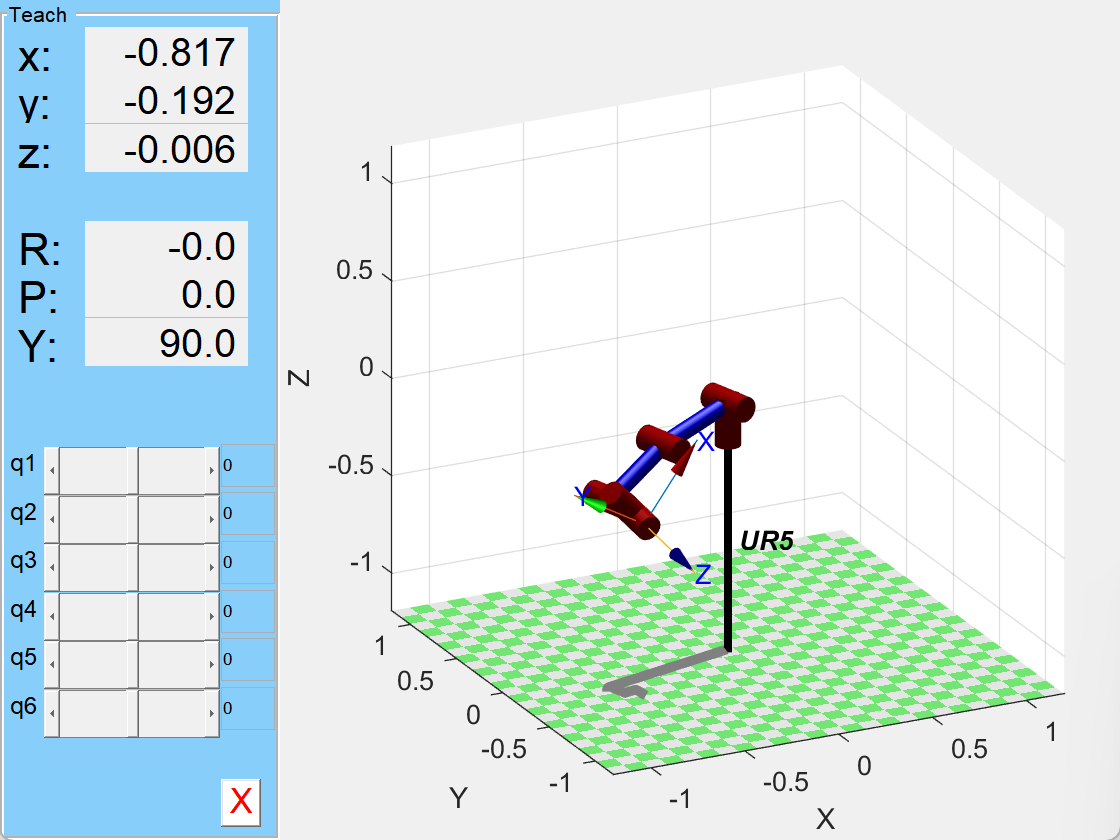
\includegraphics[width=0.5\linewidth]{fig/UR5机械臂Matlab.png}
    \caption{UR5运动学模型}
    \label{fig:UR5 for Matlab}
\end{figure}

\subsection{正运动学求解方案验证}
根据\ref{正运动学}编写正运动学求解代码,代码主要部分如下:
\begin{lstlisting}{language=C}
    function T = zhengyundongxue(theta)
      %已知关节角求变换矩阵
      a=[0,-0.42500,-0.39200,0,0,0];
      d=[0.089200,0,0,0.10930,0.09475,0.08250];
      alpha=[pi/2,0,0,pi/2,-pi/2,0];
      theta=15*ones(1,6);
      theta=theta/180*pi;
    
      T01=T_para(theta(1),d(1),a(1),alpha(1));
      T12=T_para(theta(2),d(2),a(2),alpha(2));
      T23=T_para(theta(3),d(3),a(3),alpha(3));
      T34=T_para(theta(4),d(4),a(4),alpha(4));
      T45=T_para(theta(5),d(5),a(5),alpha(5));
      T56=T_para(theta(6),d(6),a(6),alpha(6));
      
      T=T01*T12*T23*T34*T45*T56;
    end
\end{lstlisting}

运行代码后得到输出如图\ref{fig:正运动学输出结果}所示

\begin{figure}[H]
  \centering
  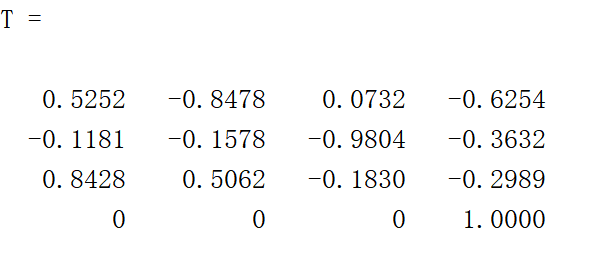
\includegraphics[width=0.5\linewidth]{fig/正运动学输出结果.png}
  \caption{正运动学输出结果}
  \label{fig:正运动学输出结果}
\end{figure}

调用Robotic Toolbox中的kfine正解函数
\begin{lstlisting}{language=C}
    p=robot.fkine(theta)
\end{lstlisting}

求得结果如图\ref{fig:Robotics Toolbox正运动学输出结果}所示
\begin{figure}[H]
  \centering
  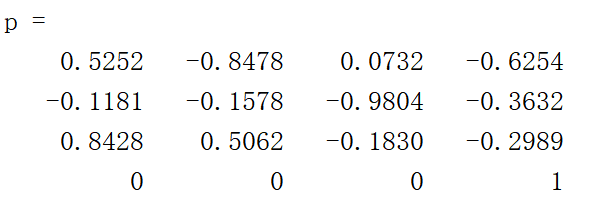
\includegraphics[width=0.5\linewidth]{fig/Robotics Toolbox正运动学输出结果.png}
  \caption{Robotics Toolbox正运动学输出结果}
  \label{fig:Robotics Toolbox正运动学输出结果}
\end{figure}

对比图\ref{fig:正运动学输出结果}和图\ref{fig:Robotics Toolbox正运动学输出结果}的结果我们可以发现,
本文所使用的正解方法与Robotics Toolbox中$fkine$函数求得的正解结果一致,验证了本文所采用的求解正运动学方案的正确性。

\subsection{逆运动学求解方案验证}
根据\ref{逆运动学}编写逆运动学求解代码,代码主要部分在附录中展示

将图\ref{fig:正运动学输出结果}正解的结果作为输入到逆解程序当中,得到8组解,结果如图\ref{fig:正运动学输出结果}所示:
\begin{figure}[H]
  \centering
  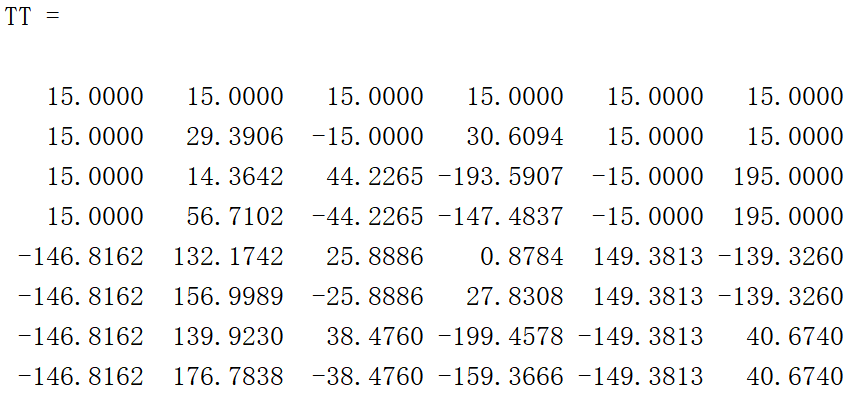
\includegraphics[width=0.7\linewidth]{fig/逆运动学输出结果.png}
  \caption{逆运动学输出结果}
  \label{fig:逆运动学输出结果}
\end{figure}

通过观察可知第一组与预设的关节角度一致,进一步我们通过Robotics Toolbox自带的求逆解公式$ikine$,求出的最优解如图\ref{fig:Robotics Toolbox逆运动学输出结果}所示。
\begin{figure}[H]
  \centering
  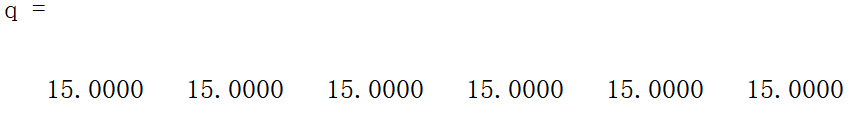
\includegraphics[width=0.7\linewidth]{fig/Robotics Toolbox逆运动学输出结果.png}
  \caption{Robotics Toolbox逆运动学输出结果}
  \label{fig:Robotics Toolbox逆运动学输出结果}
\end{figure}

进一步我们将上述求出的8组逆解的结果,作为正解的输入代入正解程序当中,得到结果一致,$^0_6T$如图\ref{fig:逆解反代}所示
\begin{figure}[H]
  \centering
  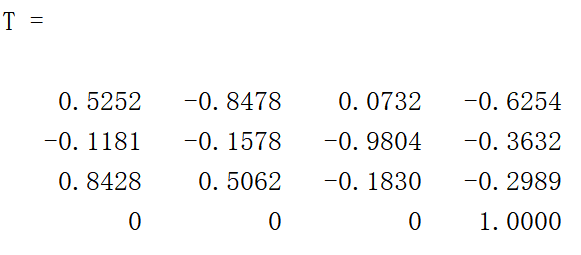
\includegraphics[width=0.5\linewidth]{fig/逆解反代结果.png}
  \caption{逆解反向求正解结果}
  \label{fig:逆解反代}
\end{figure}

通过上述步骤验证了逆解程序的正确性。

\section{本章小结}
本章主要介绍了UR5机器人的运动学建模分析以及仿真验证的过程。
首先我们通过机器人导论的基础知识学习了机器人坐标系的建立,构建了UR5机器人连杆坐标系,并写出连杆之间的齐次变换矩阵。
然后通过标准的D-H参数法来建立UR-5机器人模型,并确定其正逆运动学的求解过程,同时介绍如何确定出逆解中的最优解。
最后通过MATLAB编程实现UR5机器人的正逆运动学求解,并验证了该方案的正确性,为之后的柔顺控制打下基础。

\chapter{基于阻抗控制的柔顺控制研究}

\section{基本阻抗控制策略}

\section{自适应阻抗控制}

\section{仿真实验与分析}





\chapter{正文}
正文部分每一章应另起页书写书写,层次要清楚,内容要有逻辑性,正文一般不少于15000字。正文部分因学科、选题特点可有差异,但必须言之成理,论据可靠,严格遵循本学科国际通行的学术规范。

中文为小四号宋体,英文及数字为小四号Times New Roman,首行缩进2个字符,行间距为1.5倍。

\section{插图格式要求}
插图力求精炼,且每个插图均应有图序和图名。图序与图名位于插图下方,图序一般按章节编排,如图1-1(第一章第1个图),在插图较少时可以全文连续编序,如图10。

如一个插图由两个及以上的分图组成,分图用(a)、(b)、(c)等标出,并标出分图名。

简单文字图可用WORD直接绘制,复杂的图考虑使用相应的图形绘制软件完成,以提高图形表达质量。

插图居中排列,与上文文本之间空一行。图序图名设置为五号宋体居中,图序与图名之间空一格。

引用:图 \ref{fig:1}、图 \ref{fig:2}、图 \ref{fig:2a}、图 \ref{fig:2b} 的引用示例(见tex文件)。

\begin{figure}[H]
    \centering
    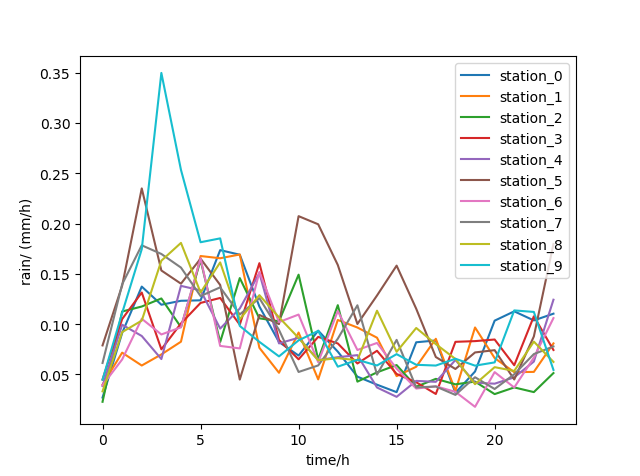
\includegraphics[width=0.5\linewidth]{fig/降水量均值分布图.png}
    \caption{每小时降水量24小时均值分布图}
    \label{fig:100}
\end{figure}

\begin{figure}[H]
    \centering
    \subcaptionbox{速度障碍集合\label{fig:2a}}
      {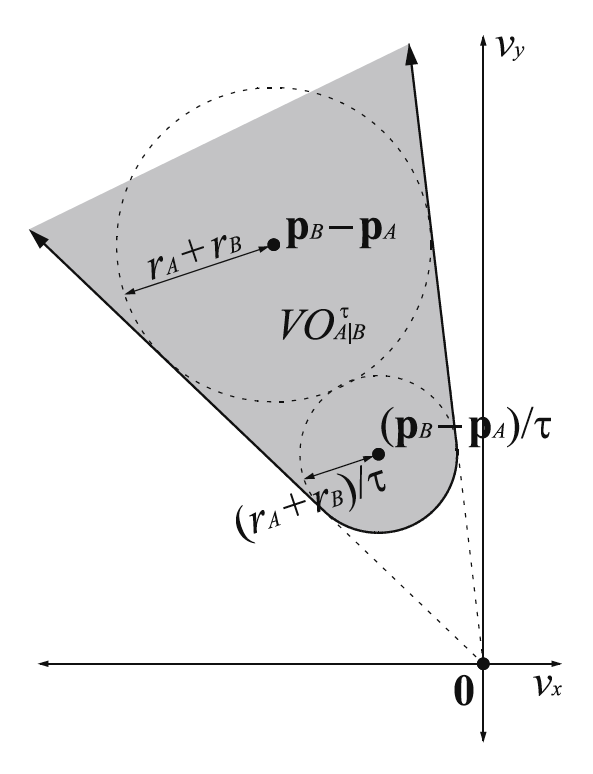
\includegraphics[width=0.3\linewidth]{fig/速度障碍集合.png}}
    \subcaptionbox{速度障碍集合\label{fig:2b}}
      {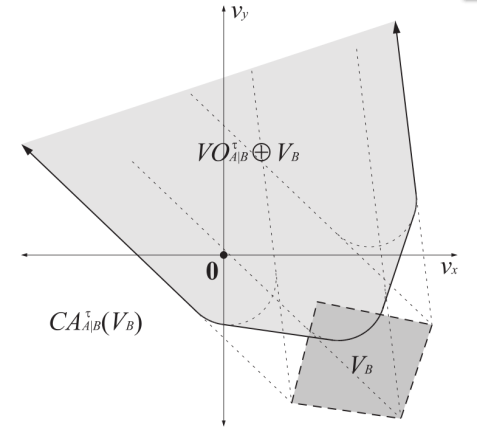
\includegraphics[width=0.4\linewidth]{fig/避免碰撞集合.png}}
    \caption{速度障碍法速度选择}
    \label{fig:200}
\end{figure}

\section{表格格式要求}
表格的结构应简洁,一律采用三线表,应有表序和表名,且表序和表名位于表格上方。表格可以逐章单独编序(如:表2.1),也可以统一编序(如:表10),采用哪种方式应和插图及公式的编序方式统一。表序必须连续,不得重复或跳跃。

表格无法在同一页排版时,可以用续表的形式另页书写,续表需在表格右上角表序前加“续”字,如“续表2.1”,并重复表头。

表格居中,边框为黑色直线1磅,中文为五号宋体,英文及数字为五号Times New Roman字体,表序与表名之间空一格,表格与下文之间空一行。需要注意必须在tabular环境前手动指定字号(见tex文件)。

引用:表 \ref{tab:1} 的引用示例(见tex文件)。

\begin{table}[H]
  \centering
  \caption{降水率分级统计}
  \label{tab:100}
  \small
  \begin{tabular}{ccc}
    \toprule
    降水率(mm/h)分级 & 该等级所占比例(\%) & 降水等级描述\\
    \midrule
    $0\le x< 0.5$ & 90.36 & 没有雨或雨很小\\
    $0.5\le x< 2.0$ & 6.41 & 小雨\\
    $2.0\le x< 5.0$ & 2.04 & 中雨\\
    $5.0\le x< 10.0$ & 0.10 & 大雨\\
    \bottomrule
  \end{tabular}
\end{table}

\section{表达式}
论文中的公式应注序号并加圆括号,序号一律用阿拉伯数字连续编序(如(28))或逐章编序(如(3.6)),编号方式应与插图、表格方式一致。序号排在版面右侧,且距右边距离相等。公式与序号之间不加虚线。

长公式在一行无法写完的情况下,原则上应在等号(或数学符号,如“+”、“-”号)处换行,数学符号在换行的行首。

公式及文字中的一般变量(或一般函数)(如坐标X、Y,电压V,频率f)宜用斜体,矢量用粗斜体如S或白斜体上加单箭头,常用函数(如三角函数cos、对数函数ln等)、数字运算符、化学元素符号及分子式、单位符号、产品代号、人名地名的外文字母等用正体。

公式排版时可选中模板中的“公式式样”,先将光标移至公式前,按“Tab”键,公式居中;再将光标移至编号前,按“Tab”键移动一个制表符位置,使公式编号右对齐。
\begin{equation}\label{eq:1000}
  V_{cell}=E_{OCV}-V_{oct}-V_{ohm}-V_{conc}
  \end{equation}
引用:公式 \eqref{eq:1000} 的引用示例(见tex文件)。

  
\section{注释}
正文中有个别名词或情况需要解释时,可加注说明,注释采用页末注(将注文放在加注页的下端)。在引文的右上角标注序号\circled{1}、\circled{2}、……,如“马尔可夫链\footnote{马尔科夫链表示}”。若在同一页中有两个以上的注时,按各注出现的先后,顺序编号。引文序号,以页为单位,且注释只限于写在注释符号出现的同页,不得隔页。

注释采用小五号宋体,英文及数字为小五号Times New Roman字体,利用“引用”插入脚注功能插入。

\chapter{总结与展望}
\section{工作总结}
最后一章结论与展望着重总结论文的创新点或新见解及研究展望或建议。

结论是对论文主要研究结果、论点的提炼与概括,应准确、简明、完整、有条理,使人看后就能全面了解论文的意义、目的和工作内容。主要阐述自己的创造性工作及所取得的研究成果在本学术领域中的地位、作用和意义。

结论要严格区分自己取得的成果与导师及他人的科研工作成果。在评价自己的研究工作成果时,要实事求是,除非有足够的证据表明自己的研究是“首次”的、“领先”的、“填补空白”的,否则应避免使用这些或类似词语。

\section{工作展望}
展望或建议,是在总结研究工作和现有结论的基础上,对该领域今后的发展方向及重要研究内容进行预测,同时对所获研究结果的应用前景和社会影响加以评价,从而对今后的研究有所启发。

\nocite{*}
\bibliographystyle{gbt7714-numerical}
\bibliography{reference.bib}



\appendix
\chapter{附录名称}
对于一些不宜放入正文中、但作为毕业设计(论文)又不可残缺的组成部分或具有重要参考价值的内容,可编入毕业设计(论文)的附录中,例如,正文内过于冗长的公式推导、方便他人阅读所需的辅助性数学工具或表格、重复性数据和图表、非常必要的程序说明和程序全文、关键调查问卷或方案等。

附录的格式与正文相同,如有多个附录需依顺序用大写字母A,B,C,……编序号,如附录A,附录B,附录C,……。只有一个附录时也要编序号,即附录A。每个附录应有标题,如:“附录A 参考文献著录规则及注意事项”。

附录一般与论文全文装订在一起,与正文一起编页码。


\begin{acknowledgement}
四年的时光转瞬即逝,虽然我的大学生活到这里结束了,但是我的人生路还很漫长,我还有很多东西需要学习。
回想我刚进入大学的时候,还是一个懵懂的少年,希望自己能在大学拓展自己各方面的能力,丰富自己的生活。
然而突如其来的疫情,让我的大学生活发生了巨大的变化,也许不是那么精彩,但让人难以忘怀。
在大学里面遇到的每一个老师,每一个同学,或许是他们一个鼓励的眼神,或许是他们一句温暖的话语,一点一滴,构成了我的大学生活。

回想过去,我首先要感谢的是我的指导老师李俊教授。李老师为人方正,严谨细致。在学术方面能给予我细致入微的指导,在生活方面也给了我很大的鼓励。
在本篇论文的选题、开题、理论研究、实验设计方面,李老师严谨的学术态度,都让人印象深刻,为我的研究工作产生了巨大的影响。

同时我也要感谢我朱战宸学长,作为研究生学长,他在我做毕设实验期间给了我很多帮助,在理论方面给予我指导,在硬件方面指导我如何使用实验室的机器人。

此外,我还要感谢我的辅导员成曦老师和武丽佳老师,他们在我的生活和学业方面给了很多帮助。感谢赵剑锋书记,在我最迷茫的大三生活中给我指明了方向。
感谢我的室友张燕坤、邢逸飞、洪伟航、郑帅、张耀祖,感谢他们在生活和学习方面的照顾,陪我度过了四年的大学时光。

在这里我还要感谢党和国家,在疫情期间各方协调,全面统筹,让我能够安心的度过三年的疫情时光。疫情消散,我们的未来是光明的,随着国家的不断发展,我也要为国家的发展贡献自己的一份力

最后,我要感谢父母和家人,在我大学的四年生活中,一直在背后默默的付出和支持。他们让我明白了学习的重要性,正是因为有他们的关心,我才能顺利完成学业。

感谢这四年里遇到的人和事,路漫漫其修远兮,吾将上下而求索,在以后的生活当中,我会珍惜这段属于我的美好时光,继续前进,继续奋斗,实现自己的人生梦想。
\end{acknowledgement}
\end{document}